\subsection{Algorithm description}
 \subsubsection{Algorithm context}
This algorithm aims to provide a partition to any k-connected graph, given any partition sizes and roots as defined in the following.

\paragraph{Algorithm input}
 \begin{description}
  \item [INPUT:] \hfill \\
    \begin{enumerate}
    \item $G = (V, E)$ a $k$-connected graph 
      \begin{figure}[H]
	\begin{center}
	  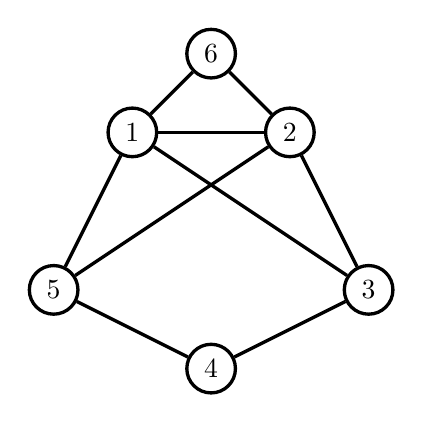
\begin{tikzpicture}
  \node[draw,circle, very thick] (A) at (1,3) {1};
  \node[draw,circle, very thick] (B) at (3,3) {2};
  \node[draw,circle, very thick] (C) at (4,1) {3};
  \node[draw,circle, very thick] (D) at (2,0) {4};
  \node[draw,circle, very thick] (E) at (0,1) {5};
  \node[draw,circle, very thick] (F) at (2,4) {6};
  \draw[very thick] (A) -- (B);
  \draw[very thick] (B) -- (C);
  \draw[very thick] (C) -- (D);
  \draw[very thick] (D) -- (E);
  \draw[very thick] (A) -- (C);
  \draw[very thick] (B) -- (E);
  \draw[very thick] (A) -- (F);
  \draw[very thick] (A) -- (E);
  \draw[very thick] (B) -- (F);

\end{tikzpicture}


	\end{center}
	\caption{An example of an input 3-connected graph with 6 edges}
      \end{figure}
    \item $k$
    \item $a_1, a_2 \ldots a_k$ : different vertices of $G$
    \item $n_1, n_2 \ldots n_k$ : strictly positive integers of $\sum_i n_i =  |V|$
    \end{enumerate}
    
  \end{description}

\paragraph{Algorithm output}
       \begin{description}
                \item[OUTPUT:] \hfill \\
                        A k-partition of G such that $\forall i \ in 1..k$ 
                        \begin{itemize} 
                                \item $H_i$ is a connected subgraph of $G$
                                \item $H_i \in Par, |V(H_i)| = n_i $
                                \item $a_i \in H_i $
                                \item $\forall j \in 1..k H_i \bigcap H_j = \emptyset$
                        \end{itemize}
        \end{description}
             \begin{figure}[H]
	       \begin{center}
	         
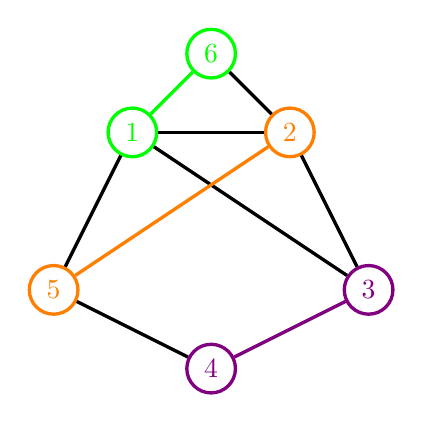
\begin{tikzpicture}
  \node[draw,circle, very thick, color=green] (A) at (1,3) {1};
  \node[draw,circle, very thick, color=orange] (B) at (3,3) {2};
  \node[draw,circle, very thick, color=violet] (C) at (4,1) {3};
  \node[draw,circle, very thick, color=violet] (D) at (2,0) {4};
  \node[draw,circle, very thick, color=orange] (E) at (0,1) {5};
  \node[draw,circle, very thick, color=green] (F) at (2,4) {6};
  \draw[very thick] (A) -- (B);
  \draw[very thick] (B) -- (C);
  \draw[very thick, color=violet] (C) -- (D);
  \draw[very thick] (D) -- (E);
  \draw[very thick] (A) -- (C);
  \draw[very thick, color=orange] (B) -- (E);
  \draw[very thick, color=green] (A) -- (F);
\draw[very thick] (A) -- (E);
  \draw[very thick] (B) -- (F);

\end{tikzpicture}


	       \end{center}
	       \caption{An example output of the 3-connected graph partition}
             \end{figure}
\paragraph{Algorithm used structures and notations}               
\label{sec:structure}
The algorithm uses its own structures and computes its own values. These are defined in this section.
\begin{description}
\item[Partition trees] represent a tree spanning over a partition of the graph $T_i  a_i$ being 
  the root of the partition. In this part of the report  a tree will refer to a partition tree, unless otherwise specified.
   \begin{figure}[H]
	\begin{center}
	  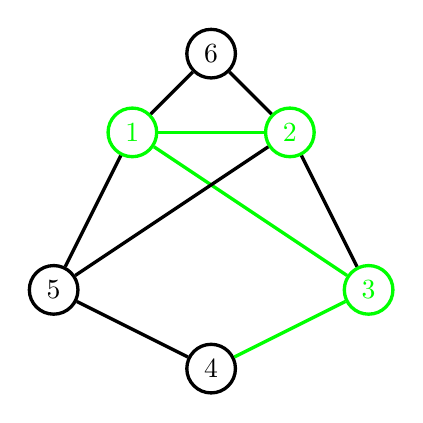
\begin{tikzpicture}
  \node[draw,circle, very thick, color=green] (A) at (1,3) {1};
  \node[draw,circle, very thick, color=green] (B) at (3,3) {2};
  \node[draw,circle, very thick, color=green] (C) at (4,1) {3};
  \node[draw,circle, very thick] (D) at (2,0) {4};
  \node[draw,circle, very thick] (E) at (0,1) {5};
  \node[draw,circle, very thick] (F) at (2,4) {6};
  \draw[very thick, color=green] (A) -- (B);
  \draw[very thick] (B) -- (C);
  \draw[very thick, color=green] (C) -- (D);
  \draw[very thick] (D) -- (E);
  \draw[very thick, color=green] (A) -- (C);
  \draw[very thick] (B) -- (E);
  \draw[very thick] (A) -- (F);
  \draw[very thick] (A) -- (E);
  \draw[very thick] (B) -- (F);

\end{tikzpicture}


	\end{center}
	\caption{An example of a partition on the input graph}
      \end{figure}
\item [Tree-Nodes] are arrays of sets of root vertices $\{a_1 \ldots a_k\}$. If $a_j \in$ Tree-node[$v$],the vertex $v$ is or has been a vertex of $T_j$. This table is used to memorize the history of the vertices membership in the partition trees. This will be later used in the algorithm to avoid endless loops and allow vertex exchange.
\begin{table}[H]
\begin{center}
  \begin{tabular}{ | l | c | c | c | c | r | }
    \hline                       
    Vertex & 1 & 2 & 3 & 4 & 5 \\
    \hline
    Set of roots & $\{a_1, a_2\}$ & $\{a_2\}$ & $\{a_3\}$ &$ \emptyset$ & $\emptyset$ \\
    \hline  
    %\caption{An example of a Tree-Node during the algorithm execution}
  \end{tabular}
\end{center}
\end{table}

\item [p] The p-value of a vertex $v$ in a tree $T_i$ the ratio $\dfrac{n_i}{|T_i|}$. The p-value is uniform in all the vertices of a tree, thus we can define the p-calue of a tree as the p-value of any of its vertices. p ensures that the trees are properly filled during the execution of the algorithm. This is due to the fact that a tree will only receive vertices from other trees which p values are lower

\end{description}

\subsubsection{Algorithm progression}

\paragraph{Step 1 : tree expansion}
The first step adds vertices that have never been in a tree before during the algorithm
Whenever there is more vertices than $n_i$ the selection of vertices to add is random. 
After applying this step to every tree we could obtain the following partition.

 \begin{figure}[H]
	\begin{center}
	  % Vertices
\SetVertexNormal[MinSize=25pt,LineColor=violet,LineWidth=3pt]%V2
\Vertex[x= 2,y=0]{a}
\SetVertexNormal[MinSize=25pt,LineColor=orange,LineWidth=3pt]%V1
\Vertex[x= 6,y=2]{e}
\Vertex[x= 8,y=0]{f}
\Vertex[x= 8,y=4]{g}
\Vertex[x=10,y=2]{h}
\SetVertexNormal[MinSize=25pt,LineColor=black,LineWidth=3pt]%Vfree
\Vertex[x= 2,y=4]{b}
\Vertex[x= 4,y=2]{c}
\Vertex[x= 0,y=2]{d}
\Vertex[x=14,y=0]{i}
\Vertex[x=14,y=4]{j}
\Vertex[x=12,y=2]{k}
\Vertex[x=16,y=2]{l}
%Cliques
\Edge[lw=1pt,color=black](a)(b)%Efree
\Edge[lw=1pt,color=black](a)(c)%Efree
\Edge[lw=1pt,color=black](a)(d)%Efree
\Edge[lw=1pt,color=black](b)(c)%Efree
\Edge[lw=1pt,color=black](b)(d)%Efree
\Edge[lw=1pt,color=black](c)(d)%Efree
\Edge[lw=3pt,color=orange](e)(f)%E1
\Edge[lw=3pt,color=orange](e)(g)%E1
\Edge[lw=3pt,color=orange](e)(h)%E1
\Edge[lw=1pt,color=black](f)(g)%Efree
\Edge[lw=1pt,color=black](f)(h)%Efree
\Edge[lw=1pt,color=black](g)(h)%Efree
\Edge[lw=1pt,color=black](i)(j)%Efree
\Edge[lw=1pt,color=black](i)(k)%Efree
\Edge[lw=1pt,color=black](i)(l)%Efree
\Edge[lw=1pt,color=black](j)(k)%Efree
\Edge[lw=1pt,color=black](j)(l)%Efree
\Edge[lw=1pt,color=black](k)(l)%Efree
%Cliques Connection
\Edge[lw=1pt,color=black](a)(f)%Efree
\Edge[lw=1pt,color=black](b)(g)%Efree
\Edge[lw=1pt,color=black](f)(i)%Efree
\Edge[lw=1pt,color=black](g)(j)%Efree

	\end{center}
	\caption{step 1 of the 3-connected graph partitioning: tree expansion}
      \end{figure}

\paragraph{Step 2 : potential swappable vertices}
\paragraph{}
The \textcolor{violet}{violet} partition needs an additional vertex that cannot be obtained through the first step. This step will let this tree expand by taking 
a vertex from an other tree.
\paragraph{}
In order to do so, the algorithm compares $p$ values of the \textcolor{violet}{violet} neighbor vertices. As mentionned in ~\ref{sec:structure} $p = \dfrac{n_i}{|V(T_i)|}$ with $T_i$ designating the current partition of the vertex. This step allows us to obtain the set of vertices adjacent to the  \textcolor{violet}{violet} partition that did not belong to this tree and with minimal $p$ value

 \begin{figure}[H]
	\begin{center}
	  % Vertices
\Vertex[x=7,y=5]{a} 
\Vertex[x=5,y=7]{b}
\Vertex[x=7,y=9]{c}
\Vertex[x=9,y=7]{d} 
\Vertex[x=0,y=2]{e}
\Vertex[x=2,y=4]{f}
\Vertex[x=4,y=2]{g}
\Vertex[x=2,y=0]{h}
\Vertex[x=10,y=2]{i}
\Vertex[x=12,y=4]{j}
\Vertex[x=14,y=2]{k}
\Vertex[x=12,y=0]{l}
%Cliques
\Edge[lw=3pt](a)(b)
\Edge[lw=3pt](a)(c)
\Edge[lw=3pt](a)(d)
\Edge[lw=1pt](b)(c)
\Edge[lw=1pt](b)(d)
\Edge[lw=1pt](c)(d)
\Edge[lw=3pt](e)(f)
\Edge[lw=3pt](e)(g)
\Edge[lw=3pt](e)(h)
\Edge[lw=1pt](f)(g)
\Edge[lw=1pt](f)(h)
\Edge[lw=1pt](g)(h)
\Edge[lw=1pt](i)(j)
\Edge[lw=1pt](i)(k)
\Edge[lw=1pt](i)(l)
\Edge[lw=1pt](j)(k)
\Edge[lw=1pt](j)(l)
\Edge[lw=1pt](k)(l)
%Cliques Connection
\Edge[lw=1pt](a)(f)
\Edge[lw=1pt](b)(g)
\Edge[lw=1pt](f)(i)
\Edge[lw=1pt](g)(j)

	\end{center}
	\caption{step 2 of the 3-connected graph partitioning: potential swappable vertices}
 \end{figure}
\paragraph{Step 3 : vertices selection}
In this step  the list of vertices obtained in the previous step is recovered.
The algorithm then choses a tree among those containing one of the latter vertices. Here the tree $T_1$ is chosen. Then among the vertices to be swapped that in addition are in this tree, the vertex with the highest degree is selected. 

 \begin{figure}[H]
	\begin{center}
	  % Vertices
\SetVertexNormal[MinSize=25pt,LineColor=violet,LineWidth=3pt]%V2
\Vertex[x= 2,y=0]{a} 
\Vertex[x= 2,y=4]{b}
\Vertex[x= 4,y=2]{c}
\Vertex[x= 0,y=2]{d}
\SetVertexNormal[MinSize=25pt,LineColor=orange,LineWidth=3pt]%V1
\Vertex[x= 6,y=2]{e}
\Vertex[x= 8,y=0]{f}
\Vertex[x= 8,y=4]{g}
\Vertex[x=10,y=2]{h}
\Vertex[x=14,y=4]{j}
\SetVertexNormal[MinSize=25pt,LineColor=black,LineWidth=3pt]%Vfree
\Vertex[x=14,y=0]{i}
\Vertex[x=12,y=2]{k}
\Vertex[x=16,y=2]{l}
%Cliques
\Edge[lw=3pt,color=violet](a)(b)%E2
\Edge[lw=3pt,color=violet](a)(c)%E2
\Edge[lw=3pt,color=violet](a)(d)%E2
\Edge[lw=1pt,color=black](b)(c)%Efree
\Edge[lw=1pt,color=black](b)(d)%Efree
\Edge[lw=1pt,color=black](c)(d)%Efree
\Edge[lw=3pt,color=orange](e)(f)%E1
\Edge[lw=3pt,color=orange](e)(g)%E1
\Edge[lw=3pt,color=orange](e)(h)%E1
\Edge[lw=1pt,color=black](f)(g)%Efree
\Edge[lw=1pt,color=black](f)(h)%Efree
\Edge[lw=1pt,color=black](g)(h)%Efree
\Edge[lw=1pt,color=black](i)(j)%Efree
\Edge[lw=1pt,color=black](i)(k)%Efree
\Edge[lw=1pt,color=black](i)(l)%Efree
\Edge[lw=1pt,color=black](j)(k)%Efree
\Edge[lw=1pt,color=black](j)(l)%Efree
\Edge[lw=1pt,color=black](k)(l)%Efree
%Cliques Connection
\Edge[lw=1pt,color=black](a)(f)%Efree
\Edge[lw=1pt,color=black](b)(g)%Efree
\Edge[lw=1pt,color=black](f)(i)%Efree
\Edge[lw=3pt,color=orange](g)(j)%E1

	\end{center}
	\caption{step 3 of the 3-connected graph partitioning: vertices selection}
      \end{figure}


\paragraph{step 4 vertices swapping}
\paragraph{}
In the last step, before repeating the loop with another tree, the vertices are swapped. To achieve this, The previously selected vertices are cut-off from their previous tree. This means that the vertex and all its children in its previous tree are removed from this partition. Because the algorithm never adds a vertex to a partition where it had already been, these vertices will be swapped to the other trees.

 \begin{figure}[H]
	\begin{center}
	  % Vertices
\SetVertexNormal[MinSize=25pt,LineColor=violet,LineWidth=3pt]%V2
\Vertex[x=4.8,y=5  ]{a} 
\Vertex[x=3.2,y=8.2]{b}
\Vertex[x=4.8,y=7  ]{c}
\Vertex[x=6.4,y=8.2]{d}
\Vertex[x=3.2,y=0  ]{f} 
\SetVertexNormal[MinSize=25pt,LineColor=orange,LineWidth=3pt]%V1
\Vertex[x=0  ,y=0  ]{e}
\Vertex[x=1.6,y=3.2]{g}
\Vertex[x=1.6,y=1.2]{h}
\Vertex[x=8  ,y=3.2]{j}
\SetVertexNormal[MinSize=25pt,LineColor=black,LineWidth=1pt]%Vfree
\Vertex[x=6.4,y=0  ]{i}
\Vertex[x=9.6,y=0  ]{k}
\Vertex[x=8  ,y=1.2]{l}
%Cliques
\Edge[lw=3pt,color=violet](a)(b)%E2
\Edge[lw=3pt,color=violet](a)(c)%E2
\Edge[lw=3pt,color=violet](a)(d)%E2
\Edge[lw=1pt,color=black](b)(c)%Efree
\Edge[lw=1pt,color=black](b)(d)%Efree
\Edge[lw=1pt,color=black](c)(d)%Efree
\Edge[lw=1pt,color=black](e)(f)%Efree
\Edge[lw=3pt,color=orange](e)(g)%E1
\Edge[lw=3pt,color=orange](e)(h)%E1
\Edge[lw=1pt,color=black](f)(g)%Efree
\Edge[lw=1pt,color=black](f)(h)%Efree
\Edge[lw=1pt,color=black](g)(h)%Efree
\Edge[lw=1pt,color=black](i)(j)%Efree
\Edge[lw=1pt,color=black](i)(k)%Efree
\Edge[lw=1pt,color=black](i)(l)%Efree
\Edge[lw=1pt,color=black](j)(k)%Efree
\Edge[lw=1pt,color=black](j)(l)%Efree
\Edge[lw=1pt,color=black](k)(l)%Efree
%Cliques Connection
\Edge[lw=3pt,color=violet](a)(f)%E2
\Edge[lw=1pt,color=black](b)(g)%Efree
\Edge[lw=1pt,color=black](f)(i)%Efree
\Edge[lw=3pt,color=orange](g)(j)%E1

	\end{center}
	\caption{step 4 of the 3-connected graph partitioning: vertices swapping}
      \end{figure}


\paragraph{Solution}
After running the loop again through the first step for $T_1 and T_5$ we obtain the output partition. The tree $T_1$ obtains \emph{F} as B belonged to $T_1$ and B is then added to $T_5$.
 \begin{figure}[H]
	\begin{center}
	  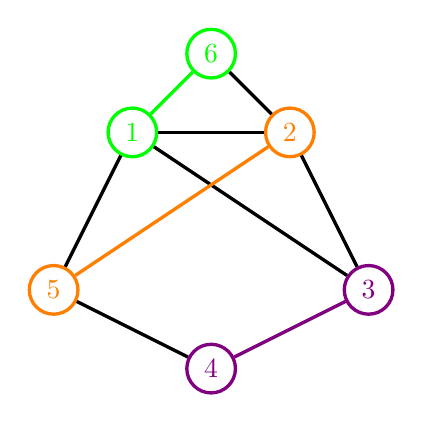
\begin{tikzpicture}
  \node[draw,circle, very thick, color=green] (A) at (1,3) {1};
  \node[draw,circle, very thick, color=orange] (B) at (3,3) {2};
  \node[draw,circle, very thick, color=violet] (C) at (4,1) {3};
  \node[draw,circle, very thick, color=violet] (D) at (2,0) {4};
  \node[draw,circle, very thick, color=orange] (E) at (0,1) {5};
  \node[draw,circle, very thick, color=green] (F) at (2,4) {6};
  \draw[very thick] (A) -- (B);
  \draw[very thick] (B) -- (C);
  \draw[very thick, color=violet] (C) -- (D);
  \draw[very thick] (D) -- (E);
  \draw[very thick] (A) -- (C);
  \draw[very thick, color=orange] (B) -- (E);
  \draw[very thick, color=green] (A) -- (F);
  \draw[very thick] (B) -- (F);
  \draw[very thick] (A) -- (E);
\end{tikzpicture}


	\end{center}
	\caption{progression toward the solution of the 3-connected graph partitioning}
      \end{figure}

